\documentclass[10pt]{article}
\usepackage{amsmath,amsfonts,times}
\usepackage{graphicx,color,tikz,pgfplots}
\usepackage[paperwidth=4.8cm,paperheight=4.2cm,lmargin=0in,rmargin=0in,tmargin=0.in,bmargin=0.in]{geometry}
\usepackage{bm}
\usetikzlibrary{arrows,shadings,shapes.arrows,decorations.pathreplacing,calc, positioning}
\usepgfplotslibrary{fillbetween}

\pgfplotsset{
  compat=newest
}

\newlength{\dx}
\setlength{\dx}{2cm}

\newlength{\dy}
\setlength{\dy}{1.cm}

\newlength{\circleRadius}
\setlength{\circleRadius}{0.95\dx}

\definecolor{outside}{rgb}{0, 1, 0}
\definecolor{cutcell}{rgb}{0, 0.5, 1}
\definecolor{inside}{rgb}{1, 0, 0}

\tikzset{
  edge/.style={thick, draw=black},
  tree/.style={thick, draw=black, densely dotted},
  bvh/.style={draw=black, minimum width=5mm, minimum height=5mm, rectangle, very thick},
  vertex/.style={circle, inner sep=0pt, minimum width=4pt, draw=black, fill=black, node contents={}},
  point/.style={circle, inner sep=0pt, minimum width=6pt, thick, draw=black, fill=white},
  root/.style={ultra thick, densely dashed, draw=black},
  left/.style={very thick, draw=black, solid, fill=blue, fill opacity=0.2},
  right/.style={very thick, draw=black, solid, fill=red, fill opacity=0.2},
}

\begin{document}
\centering
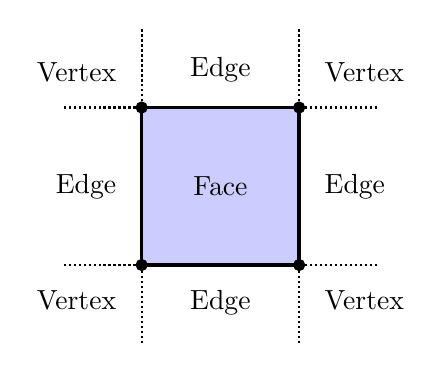
\begin{tikzpicture}

  \draw[left] (0,0) rectangle (\dx, \dx);
  
  \node (v0) at (0,0) [vertex];
  \node (v1) at (\dx,0) [vertex];
  \node (v2) at (\dx,\dx) [vertex];
  \node (v3) at (0, \dx) [vertex];

  \draw[tree] (v0) --++(-\dy, 0);
  \draw[tree] (v0) --++(0,-\dy);

  \draw[tree] (v1) --++(\dy, 0);
  \draw[tree] (v1) --++(0,-\dy);

  \draw[tree] (v2) --++(\dy, 0);
  \draw[tree] (v2) --++(0,\dy);

  \draw[tree] (v3) --++(-\dy, 0);
  \draw[tree] (v3) --++(0,\dy);

  \node[anchor=north east] at (-0.1\dx, -0.1\dx) {Vertex};
  \node[anchor=north west] at (1.1\dx, -0.1\dx) {Vertex};
  \node[anchor=south east] at (-0.1\dx, 1.1\dx) {Vertex};
  \node[anchor=south west] at (1.1\dx, 1.1\dx) {Vertex};

  \node[anchor=north] at (0.5\dx, -0.1\dx) {Edge};
  \node[anchor=west] at (1.1\dx, 0.5\dx) {Edge};
  \node[anchor=east] at (-0.1\dx, 0.5\dx) {Edge};
  \node[anchor=south] at (0.5\dx, 1.1\dx) {Edge};

  \node at (0.5\dx, 0.5\dx) {Face};
  
\end{tikzpicture}

\end{document} 
